% OpenSTS — IGARSS 2027 full paper (4 pages).
% Preamble is IEEEtran conference as a stand-in: swap it for the official IGARSS 2027
% paper-kit template once downloaded; the body below needs no other change.
% RULE: every number must appear with the same value in docs/RESULTS.md (section cited in
% the comment beside it). \tbd{} marks numbers that wait on the 3-rotation run.
% Build: tectonic paper/main.tex
\documentclass[conference]{IEEEtran}
\usepackage{amsmath,graphicx,booktabs,multirow,xcolor,tikz}
\usetikzlibrary{positioning,arrows.meta}
\usepackage[hidelinks]{hyperref}
\newcommand{\tbd}[1]{\textcolor{red}{#1}}

\begin{document}

\title{OpenSTS: An Open Pipeline for Screening AIS-Unmatched Vessels and
Ship-to-Ship Transfer Candidates in Sentinel-1 SAR}

\author{\IEEEauthorblockN{K.~Jaswanth}
\IEEEauthorblockA{Independent Researcher, Hyderabad, India\\ koppisettyjaswanth@gmail.com}}

\maketitle

\begin{abstract}
Vessels that stop broadcasting the Automatic Identification System (AIS) and meet at
sea for ship-to-ship (STS) transfers are a known route for sanctions evasion, but
monitoring them usually depends on commercial imagery and AIS feeds. We present OpenSTS,
an open pipeline built only on free data: Sentinel-1 SAR from Microsoft Planetary
Computer, Danish Maritime Authority (DMA) AIS, and Global Fishing Watch (GFW) as an
independent cross-check. Training labels are generated by matching AIS to SAR targets;
an audit of the labeler found three defects, and fixing them raised mAP50 from 0.16 to
0.38 with the detector unchanged. Five detectors trained on 339 tiles from three regions
reach vessel mAP50 of 0.51--0.56 on held-out scenes of the two added regions, against
0.11 for a single-region model, but only 0.12--0.22 when the test region is withheld
from training entirely. Over three months in the Gulf of Oman, the pipeline
flags 168 AIS-unmatched vessels of 100\,m or longer that GFW's own SAR detections also
leave unmatched, and 12 AIS-unmatched STS candidates across two regions in three
evidence tiers. No candidate is confirmed: Sentinel-2 images taken hours to days later
neither confirm nor rule out any of 12 checked. Code and data are public at
\tbd{\url{https://github.com/Jaswanth-K1210/smugglers}, DOI~10.5281/zenodo.XXXXXXX}.
\end{abstract}

\begin{IEEEkeywords}
SAR, Sentinel-1, ship detection, AIS, ship-to-ship transfer, open data
\end{IEEEkeywords}

\section{Introduction}
\label{sec:intro}
% DRAFT by Claude from the notes: rewrite in your own words; check every claim
% about the cited papers against the papers themselves.
Ships switch off, lose or never fit the Automatic Identification System (AIS), and
ship-to-ship (STS) transfers at sea are one way cargo changes hands outside port
controls, a concern for sanctions enforcement and illegal fishing alike. AIS alone
reveals transshipment only when both vessels broadcast \cite{miller2018}. Synthetic
aperture radar (SAR) images ships through cloud and at night whether or not they
transmit, and Sentinel-1 \cite{torres2012} provides it free of charge, whereas
commercial SAR and AIS feeds are costly for researchers and small agencies.

A ship that radar sees and AIS does not is not evidence of concealment: the gap can
come from reception, coverage, equipment failure or processing. We therefore call such
targets \emph{AIS-unmatched}, never ``dark'', and report them as candidates with the
evidence for each, not as detections of wrongdoing.

The closest work, Ballinger \cite{ballinger2024}, detects dark STS transfers in
satellite imagery with deep learning. OpenSTS takes the same goal in a different
direction: (i) only free data end to end, including AIS outside Denmark from Global
Fishing Watch (GFW); (ii) an audited AIS-to-SAR auto-labeler whose effect on accuracy is
measured; and (iii) graded evidence tiers with an independent GFW cross-check instead
of a binary label.

Contributions: (1) an open, reproducible pipeline and dataset using only free data;
(2) an audit of AIS-based auto-labeling, showing that three label defects outweigh the
choice of detector, and a leave-one-region-out test showing that scene-level splits
overstate accuracy on unseen sea areas; (3) a multi-region screening of AIS-unmatched vessels and STS
candidates with tiered evidence and stated limits.

\section{Related Work}
\label{sec:related}
% DRAFT by Claude: rewrite; cut first if over 4 pages.
SAR ship detection is commonly benchmarked on SSDD \cite{li2017} and HRSID
\cite{wei2020}, small chips with manual boxes, and on xView3-SAR \cite{paolo2022},
which pairs full Sentinel-1 scenes with AIS-derived labels to find vessels that do not
broadcast. Paolo et al.\ \cite{paolo2024} extended this to a global map of vessels
missing from public AIS. On the AIS side, GFW, building on \cite{kroodsma2018},
publishes encounter events between broadcasting vessels, and Miller et
al.\ \cite{miller2018} characterised transshipment from AIS alone; both see only
vessels that transmit. Ballinger \cite{ballinger2024} combines the two views for STS;
OpenSTS differs as set out above and adds tiers that state what the radar shows.

\section{Data and Method}
\label{sec:method}


\textbf{Data.} Sentinel-1 IW GRDH VV scenes are read from Microsoft Planetary Computer
\cite{pc2022}, warped to UTM at 10\,m and cut into $1024\times1024$ tiles. Three areas
are used: the Skagen anchorage, Denmark (AIS from DMA daily files); the Fujairah
anchorage, Gulf of Oman; and the Gulf of Laconia, Greece (AIS from GFW hourly presence
\cite{kroodsma2018}). Scenes span July--September 2026. % RESULTS setup, §4b–4e

\begin{figure}[t]
\centering
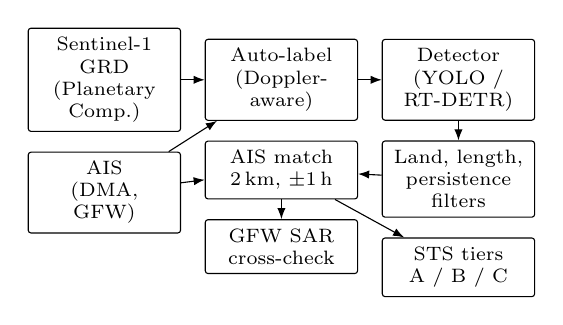
\begin{tikzpicture}[node distance=2.5mm and 3mm, font=\scriptsize,
  b/.style={draw, rounded corners=1pt, align=center, minimum height=6mm, text width=17mm},
  a/.style={-{Latex[length=1.4mm]}}]
\node[b] (s1) {Sentinel-1 GRD\\(Planetary Comp.)};
\node[b, below=of s1] (ais) {AIS\\(DMA, GFW)};
\node[b, right=of s1] (lab) {Auto-label\\(Doppler-aware)};
\node[b, right=of lab] (det) {Detector\\(YOLO / RT-DETR)};
\node[b, below=of det] (flt) {Land, length,\\persistence filters};
\node[b, below=of lab] (mat) {AIS match\\2\,km, $\pm$1\,h};
\node[b, below=of mat] (gfw) {GFW SAR\\cross-check};
\node[b, below=of flt] (sts) {STS tiers\\A / B / C};
\draw[a] (s1) -- (lab); \draw[a] (ais) -- (lab); \draw[a] (lab) -- (det);
\draw[a] (det) -- (flt); \draw[a] (flt) -- (mat); \draw[a] (ais) -- (mat);
\draw[a] (mat) -- (gfw); \draw[a] (mat) -- (sts);
\end{tikzpicture}
\caption{OpenSTS pipeline.}
\label{fig:pipeline}
\end{figure}

\textbf{Auto-labeling and its audit.} Each AIS track is interpolated to the acquisition
second and boxed on the SAR target it falls on. Inspecting validation predictions
exposed three defects (Table~\ref{tab:labelfix}). (i) Two vessels moored together form
one blob at 10\,m, and received both two \emph{vessel} boxes and one \emph{sts} box on
the same pixels, so \emph{sts} could not be learned; such pairs are now labeled
\emph{sts} only. (ii) Moving ships are displaced in azimuth by the Doppler shift
\cite{raney1971}: over 854 labels the median box-to-AIS offset grows from 61\,m below
1\,kn to 376\,m above 10\,kn, about 60\,m per knot, so a fixed 600\,m search dropped fast
ships or boxed the wrong target. The radius is now $600\,\mathrm{m} + 60\,\mathrm{m/kn}
\times \mathrm{SOG}$, capped at 2\,km. (iii) Boxes whose length falls outside
0.5--2$\times$ the AIS length are dropped. The Skagen set shrank from 854 vessel / 63 sts
boxes on 223 tiles to 516 / 64 on 170 tiles: fewer labels, but consistent ones. % §1

\textbf{Multi-region training.} Oman and Laconia have no labeler-grade AIS, so
detections of the Skagen model that a GFW AIS identity confirms become \emph{vessel}
pseudo-labels; tiles holding any unmatched or \emph{sts} detection are left out, so a
possible ship is never taught as background. This uses GFW AIS positions, never GFW
classifications, and is disclosed. The set has 339 tiles (Skagen 170, Oman 140, Laconia
29), split by scene, never by tile (284 train / 55 validation). Five detectors
\cite{ultralytics,yolo26,rtdetr} are trained for 80 epochs at 1024\,px with SAR-appropriate
augmentation (no color jitter, full rotation, flips). % §6, §6b

\textbf{Screening.} Detections pass land (1\,km), length and static-infrastructure
masks, per-scene de-duplication (150\,m) and a persistence check: an unmatched position
recurring across scenes is a structure, not a vessel. A detection is
\emph{AIS-unmatched} if no AIS identity lies within 2\,km and $\pm$1\,h, a deliberately
generous window so that a miss is meaningful and Doppler offset cannot cause one. As an
independent check, it is also tested against GFW's own Sentinel-1 detections
\cite{paolo2024}. We do not call these vessels ``dark'': AIS absence may be reception,
coverage, equipment failure or processing. % §4, §4b, §4c

\textbf{STS candidates.} Two-hull configurations are graded by evidence: \textbf{A} two
hulls $\le$150\,m apart (moored together); \textbf{B} 150--500\,m apart; \textbf{C} one
hull wider than the 99th-percentile beam of AIS-matched ships of its length band
(disabled for bands with fewer than 50 matched ships). AIS is counted per candidate as
radar hulls within 1\,km minus AIS identities within 1.75\,km. A \emph{one-hull rule}
prevents one long ship detected twice from counting as a pair: two detections are two
ships only if each sits on its own bright hull, or if they lie side by side rather than
along one hull's axis; two parts up to 200\,m apart count as one hull with a dark gap when each points along the
line between the detections or is round, and at least one is long. % §4d, §4g

\section{Experiments and Results}
\label{sec:results}

\begin{table}[t]
\caption{Label audit: YOLOv8n before and after the three fixes (mAP50). Held-out scenes
differ slightly between runs, so the comparison is indicative.}
\label{tab:labelfix}
\centering\small
\begin{tabular}{lccc}
\toprule
Labels & Vessel & STS & Overall \\
\midrule
Original & 0.311 & 0.000 & 0.156 \\
Fixed    & \textbf{0.419} & \textbf{0.341} & \textbf{0.380} \\
\bottomrule
\end{tabular}
\end{table}

\textbf{Label quality outweighs architecture.} Fixing the labels doubled overall mAP50
(Table~\ref{tab:labelfix}). On the same fixed Skagen labels, four detector families
differ by at most 0.054 in overall mAP50 (0.348--0.402), within the $\pm$0.05
epoch-to-epoch swing of a 37-tile validation set; RT-DETR-l stands out only in recall
(0.66 vs.\ 0.30 for YOLOv8n). % §2, §3

\begin{table}[t]
\caption{Vessel mAP50 on the same held-out scenes. ``New'' = 25 tiles from Oman and
Laconia; CPU time per 1024\,px tile.}
\label{tab:detectors}
\centering\footnotesize
\setlength{\tabcolsep}{4pt}
\begin{tabular}{lcccc}
\toprule
Model & New & Rec.\ new & Skagen & CPU s \\
\midrule
RT-DETR-l (Skagen) & 0.113 & 0.311 & 0.367 & -- \\
\midrule
RT-DETR-l & 0.512 & 0.571 & \textbf{0.475} & 3.49 \\
YOLOv8n   & 0.532 & 0.526 & 0.329 & \textbf{0.30} \\
YOLO11n   & 0.523 & 0.543 & 0.402 & 0.40 \\
YOLO12n   & 0.546 & \textbf{0.612} & 0.361 & 0.79 \\
YOLO26n   & \textbf{0.558} & 0.547 & 0.386 & 0.31 \\
\bottomrule
\end{tabular}
\end{table}

\textbf{Pseudo-labels help within their regions.} The Skagen-only detector scores
0.113 vessel mAP50 on held-out scenes of the new regions; adding AIS-confirmed
pseudo-labels from those regions lifts it to 0.512 (Table~\ref{tab:detectors}). All five multi-region detectors lie within 0.05 of
each other on the new regions, inside the noise of 25 tiles, so speed decides
deployment: YOLO26n is served (0.31\,s per tile on CPU), RT-DETR-l is the accuracy
reference. Precision on new-region tiles reads low because ships the Skagen model
missed are unlabeled there. % §6, §6b

\textbf{Unseen regions.} Table~\ref{tab:loro} trains on two regions and tests on all
tiles of the third. Withholding a whole region cuts vessel mAP50 to 0.122--0.140 in Oman
and 0.183--0.217 in Laconia, against 0.51--0.56 for held-out scenes of the same regions:
a scene split measures generalisation within a region, not to a new area of sea. Oman,
the densest anchorage (1590 boxes on 140 tiles), is hardest, and its labels miss ships
the Skagen detector missed, so its score is a lower bound. Skagen held out scores
0.428--0.509, but the Oman and Laconia pseudo-labels came from a Skagen-trained detector,
so Skagen is not fully unseen upstream. No family wins consistently; Laconia's 37 test
boxes are too few to separate them.

\begin{table}[t]
\caption{Leave-one-region-out vessel mAP50: trained on the other two regions, tested
on all tiles of the named one (170 / 140 / 29 tiles).}
\label{tab:loro}
\centering\small
\begin{tabular}{lccc}
\toprule
Test region & Skagen & Oman & Laconia \\
\midrule
YOLO26n   & 0.428 & 0.122 & \textbf{0.217} \\
RT-DETR-l & \textbf{0.509} & \textbf{0.140} & 0.183 \\
\bottomrule
\end{tabular}
\end{table}

\begin{table}[t]
\caption{AIS-unmatched screening. Skagen: July--August, months the detector never saw;
Oman and Laconia: July--September. +GFW: also unmatched in GFW's SAR detections. ``Reported'' criteria differ by region
(see text).}
\label{tab:unmatched}
\centering\footnotesize
\setlength{\tabcolsep}{3pt}
\begin{tabular}{lccccc}
\toprule
Region & Checked & Matched & Unmatched & +GFW & Reported \\
\midrule
Skagen  & 1,297 & 96.7\,\% & 29  & --  & 16 \\
Oman    & 7,417 & 93.1\,\% & 512 & 213 & 168 \\
Laconia & 123   & 47.2\,\% & 65  & 25  & 25 \\
\bottomrule
\end{tabular}
\end{table}

\textbf{AIS-unmatched vessels.} Table~\ref{tab:unmatched}. In Skagen, where coastal AIS
reception is good, 96.7\,\% of ships match AIS; all 29 unmatched were inspected and 16
are strong or plausible vessel-like targets. In Oman, the unmatched rate is
$\sim$3$\times$ Skagen's; we report the 168 that are $\ge$100\,m (where AIS carriage is
mandatory for most ships) and also unmatched in GFW's detections. The 30 highest-ranked
were inspected and all 30 are unambiguous large ships of 134--388\,m, consistent with
Aframax to VLCC tanker sizes. Fujairah is among the densest anchorages in the world,
where satellite AIS messages collide, which is why the GFW cross-check is required. In
Laconia, 25 unmatched ships are also unmatched by GFW. % §4b, §4c, §4e
% NOTE: Laconia "Matched" 47.2 % = 58/123, computed from §4e counts.

\textbf{STS candidates.} The first Oman pass produced 41 AIS-unmatched STS candidates
without a GFW encounter event; inspecting the top 30 found 4 strong and 9 plausible
two-vessel configurations, but 12 were one hull detected twice. The one-hull rule
reduced the set to 21 in Oman, and inspection showed most tier-C ``over-wide'' hulls
were one bright ship whose thin sidelobe cross was measured as beam, and two tier-B
pairs were one tanker whose bright bow and superstructure image apart; the Oman
tier-A pair was two boxes on one tanker. Measuring beam
after removing features thinner than 30\,m, and joining in-line parts up to 200\,m
apart, left \textbf{11 in Oman} (B\,7, C\,4) and \textbf{1 in Laconia} (tier A,
two parallel hulls with no AIS on either).
GFW lists only 2 encounter events in the Oman area for the period, so it can neither
confirm nor rule out these candidates. \tbd{Provisional: 34 newly over-wide detections
await AIS counting (GFW presence API down).} % §4d, §4e, §4g

\textbf{Optical check.} For 12 candidates (10 Oman, 2 Laconia, selected before the
one-hull rule), the nearest clear Sentinel-2 L2A image within $\pm$5 days shows no pair
at the spot. Sentinel-2 passes hours from the radar time (median gap $\sim$40\,h in
Oman), and moored transfers last hours to a day or two, so an empty sea is the expected
outcome either way: no confirmation and no contradiction. % §4f

\begin{figure}[t]
\centering
\IfFileExists{fig2.pdf}{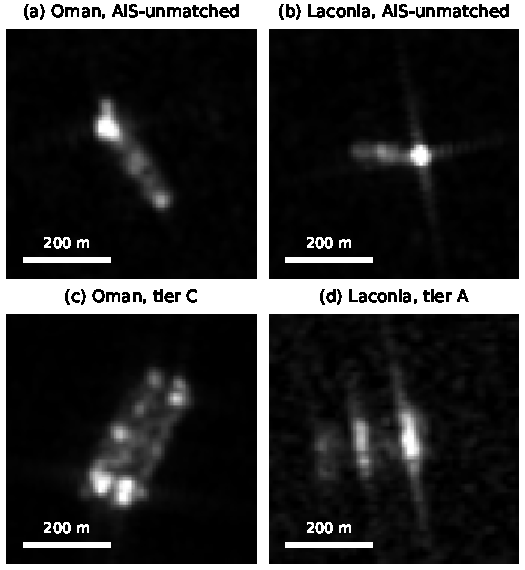
\includegraphics[width=\columnwidth]{fig2.pdf}}{%
\fbox{\parbox{0.95\columnwidth}{\centering\vspace{12mm}\tbd{fig2.pdf: run notebook
07\_tierc section 7, copy darksts/fig2.pdf into paper/}\vspace{12mm}}}}
\caption{Sentinel-1 VV chips: AIS-unmatched vessels also unmatched by GFW in (a) Oman
and (b) Laconia; (c) an Oman tier-C over-wide hull; (d) the Laconia tier-A pair, two
parallel hulls with no AIS on either.}
\label{fig:examples}
\end{figure}

\section{Limitations and Conclusion}
\label{sec:conclusion}
Detection accuracy is modest (vessel mAP50 $\approx$0.5 within the training regions,
0.12--0.22 in a region withheld from training) and measured on small sets (25--37
validation tiles, 11 STS instances); the learned \emph{sts} class is
unreliable on the multi-region split, so STS candidates come from geometry, not the
classifier. Pseudo-labels in Oman and Laconia are confirmed with GFW AIS, so GFW is not
fully independent there. Recall is near zero within 3\,km of shore. A single C-band VV
sensor at 10\,m merges rafted hulls and cannot see cargo, and \textbf{no STS candidate
has been confirmed}: confirmation needs optical imagery close to the radar time, which
free sensors rarely provide. OpenSTS's contribution is therefore openness, low cost and
verifiable evidence, not accuracy: the released code, labeled tiles and tier
definitions let others reproduce every number and test the candidates with better data.

\section*{Acknowledgment}
Contains modified Copernicus Sentinel-1 and Sentinel-2 data (2026). AIS data from the
Danish Maritime Authority and Global Fishing Watch. Imagery accessed through Microsoft
Planetary Computer.

\bibliographystyle{IEEEtran}
\bibliography{refs}

\end{document}
